\section*{20-05 - Galassie2}
\subsection*{Struttura della galassia}
\begin{figure}[h]
    \centering
    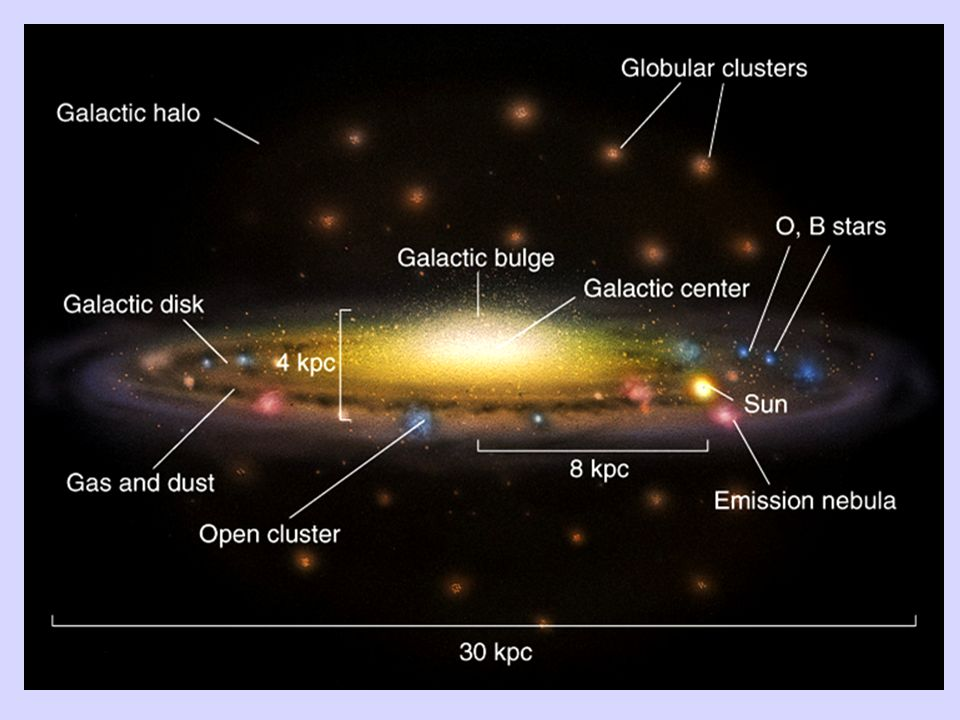
\includegraphics[width=.8\columnwidth]{images/strutturagalassia.jpg}
    \caption{Principali strutture di una galassia.}
    \label{fig:strutturagalassia}
\end{figure}
\noindent
Nella Figura \ref{fig:strutturagalassia} vediamo una rappresentazione della Via Lattea in cui sono indicate le principali strutture che la compongono. Il disco, cioè la parte più sottile, ha un raggio dell'ordine di 20 kpc. Come si può immaginare, è difficile parlare di estensione poiché nel punto in cui finiscono le stelle ci sono ancora diversi kpc in cui si estendono i gas del ISM. Sul disco abbiamo stelle di diverse generazioni ed il ISM (polvere, HI e nubi molecolari). La zona sferoidale è chiamata alone, dove troviamo gli ammassi globulari. Si distingue dal disco perché le stelle che lo popolano sono solo antiche ($\gtrsim 10^{10}\um{yr}$) e sono tutte povere di metalli. Le stelle che hanno queste caratteristiche prendono il nome di stelle di Popolazione 2. Le altre prendono il nome di stelle di popolazione 2. Nella zona centrale troviamo il bulge, un rigonfiamento che ha un raggio dell'ordine del kpc. Ha una grande densità di stelle vecchie e ricche di metallo e di ISM.\\

\subsection*{Contributo di gas ionizzato - Nubi di HII}
Dobbiamo aspettarci il contributo di un gas ionizzato. Sappiamo che le stelle nascono dalla contrazione delle nubi di gas interstellare. Una volta che accendiamo la stella, cosa succede al gas che la circonda?\\
Sappiamo che l'energia per ionizzare l'idrogeno neutro $\ce{HI}$ deve essere $E\ge E_0=13.6\um{eV}$. A quest'energia corrisponde una $\lambda\le\lambda_0 = 912$ \AA. Le stelle emettono un numero significativo di fotoni con questa lunghezza d'onda? Dipenderà dalla temperatura effettiva. Guardando i tipi spettrali, scopriamo che le stelle in grado di produrre fotoni in grado di ionizzare l'HI sono quelle di tipo O e di tipo B ($T_{\text{eff}}>20000\um{K}$). Sappiamo che nel gas abbiamo anche He ma l'energia di prima ionizzazione dell'elio è abbastanza più alta da rendere la sua ionizzazione decisamente più rara (sono poche le stelle abbastanza massicce). Avremo un processo del tipo
\[
    \ce{HI + {\gamma}  -> HII + e-}
\]

\begin{figure}[h!]
    \centering
    \resizebox{.4\columnwidth}{!}{%
        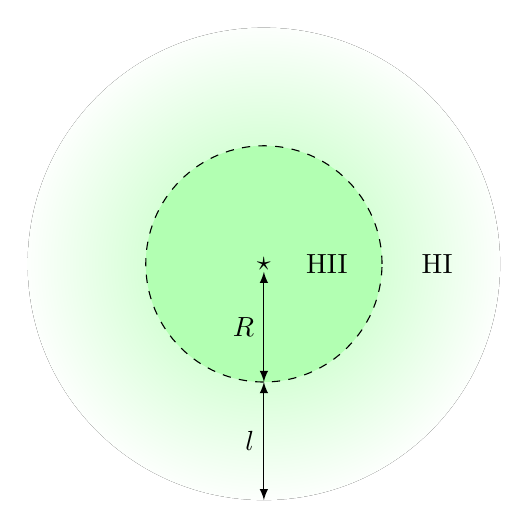
\begin{tikzpicture}
            \fill[even odd rule,inner color=green!30,outer color=green!1] (0,0) circle (3);
    %        \fill[blue!5] (0,0) circle (3);
            \filldraw[fill=green!30,dashed] (0,0) circle (1.5);
            % \filldraw[black] (0,0) circle (1pt) node[above] {Star};
            \draw[>=latex, <->, black] (0,-0.1) -- (0,-1.5) node[left, pos=.5]{$R$};
            \draw[>=latex, <->, black] (0,-1.5) -- (0,-3) node[left, pos=0.5]{$l$};
            \node(h1) at (.8,0){HII};
            \node(h2) at (2.2,0){HI};
            \node(stella) at (0,0){$\star$};
        \end{tikzpicture}
    }
    \caption{Distribuzione dell'idrogeno attorno ad una stella.}
    \label{fig:idrogenostelle}
\end{figure}
Vogliamo sapere quanto è grande la regione HII (vedi Figura \ref{fig:idrogenostelle}). Il primo a studiare questo tipo di processo fu Strongren nel 1939. Fece due assunzioni: la stella, massiccia, arriva molto rapidamente alla fase di sequenza principale (che non è vero, sappiamo che ci vogliono decine di migliaia di anni), e che il mezzo che circondava la stella appena nata è omogeneo. Con queste due assunzioni, la regione prende una forma sferica che prende il nome di Sfera di Strongren. Supponiamo che ad un certo istante la stella abbia ionizzato la regione di raggio $R$. Un fotone ionizzante emesso dalla stella attraverserà la zona già ionizzata praticamente indisturbatamente. Vediamo perché. In questa regione abbiamo soltanto protoni ed elettroni, quindi il tipo di interazione tra fotone e mezzo sarà di scattering elettronico. Sappiamo che a queste energie saremo nel limite non relativistico e che quindi avremo uno scattering Thomson, che è molto piccola ($\sigma_\text{T}=6.65\times10^{-25}\um{cm}^2$). Il cammino libero medio di un fotone ionizzante sarà
\begin{equation}
    l_\text{T} = \frac{1}{n_e\sigma_\text{T}} \gg R
\end{equation}
dato che $n_e\sim n_\text{H}\approx10^3\um{cm}^{-3}$ e che quindi $l_\text{T}\approx10 \um{pc}$. Di conseguenza il fotone ionizzante entra nella zona di HI, in cui invece ha una sezione d'urto $\sigma \approx 10^{-17}\um{cm}^2$ e quindi $l=\frac{1}{n_\text{HI}\sigma}\approx 10^{-3}\um{pc}$. Quindi questo fotone non riuscirà mai ad uscire dalla regione di HI. Quindi per ogni fotone ionizzante prodotto si avrà una ionizzazione nella regione di idrogeno neutro, che produce uno spostamento del fronte di ionizzazione, sta aumentando $R$. Fino a quando aumenterà? Presa una shell di raggio $dR$, avremo un numero di atomi nella shell pari a 
\begin{equation}
    dN_\text{H} = 4\pi R^2 n_\text{HI} dR
\end{equation}
Di quanto riuscirà a progredire il fronte di ionizzazione dipernderà dal numero di fotoni ionizzanti emessi nell'unità di tempo. Sapendo che ciascun fotone ionizzante ionizzerà un atomo di idrogeno possiamo scrivere 
\begin{equation}
    dN_i= dN_\text{H} \Rightarrow \frac{dN_i}{dt} = 4\pi R^2 n_\text{HI} \frac{dR}{dt}.
    \label{eq:ionizzanti}
\end{equation}
Questa situazione non può andare avanti in eterno. Prima o poi gli atomi che si trovano nella regione ionizzata HII si ricombineranno e formeranno di nuovo un atomo di idrogeno neutro. Quando questo succederà l'Eq. \ref{eq:ionizzanti} non sarà più valida perché i fotoni prodotti dalla stella verranno intercettati dagli atomi ricombinati. Di conseguenza dobbiamo aggiungere un altro termine che tenga conto dei fotoni intercettati. Se conosciamo il rate di ricombinazione ($r=n_pn_e\alpha$), scriviamo
\begin{equation}
    \frac{dN_i}{dt} = 4\pi R^2 n_\text{HI} \frac{dR}{dt}+ \frac{4}{3}\pi R^3 n_pn_e\alpha
    \label{eq:ricombinati}
\end{equation}
con $\alpha=\langle\sigma_rv\rangle$, in cui $\sigma_r$ è la sezione d'urto della ricombinazione. Man mano che la sfera aumenta di raggio crescerà tanto il termine di destra fino a diventare dominante. Quando ciò avviene deve succedere
\begin{equation}
    \frac{dR}{dt}=0 \Rightarrow \frac{dN_i}{dt}=\frac{4}{3}\pi R_\text{S}^3 n_pn_e\alpha
\end{equation}
e la zona non può più aumentare di raggio. $R_\text{S}$ prende il nome di raggio di Strongren e, riscrivendo, vale
\begin{equation}
    R_\text{S}=\left(\frac{3}{4\pi n_pn_e\alpha}\frac{dN_i}{dt}\right)^{\frac{1}{3}}.
\end{equation}
Le dimensioni di questo raggio dipenderanno dalla stella, particolarmente dal numero di fotoni ionizzanti e quindi dalla luminosità ad una certa frequenza. Scriviamo che
\begin{equation}
    \frac{dN_i}{dt} = \int_{\nu_{0}}^{\infty} \frac{L_\nu}{h\nu}d\nu,\quad h\nu=13.6\um{eV}
\end{equation}
Quindi se conosciamo lo spettro della stella possiamo calcolare quanti fotoni hanno l'energia sufficiente a ionizzare un atomo di idrogeno e quindi calcolare il raggio della zona HII. Per curiosità, una stella di tipo O5V produce ${dN_i}/{dt}\approx 3\times10^{49}\um{s}^{-1}$.\\
Continua pag. 185 Choudhuri con bremsstrahlung e gas coronale.